As things currently stand, the gateway can not be connected to a secured network.
While the network can have a WPA2 password, it can not have a firewall or any additional security measures.
You can test your internet connection from the gateway by \lstinline[language=sh]{ping}ing Google's \lstinline[language=sh]{8.8.8.8} server.
If you see results like those shown in \cref{fig:ping}, then your network is sufficiently exposed.
\begin{figure}[ht]
  \centering
  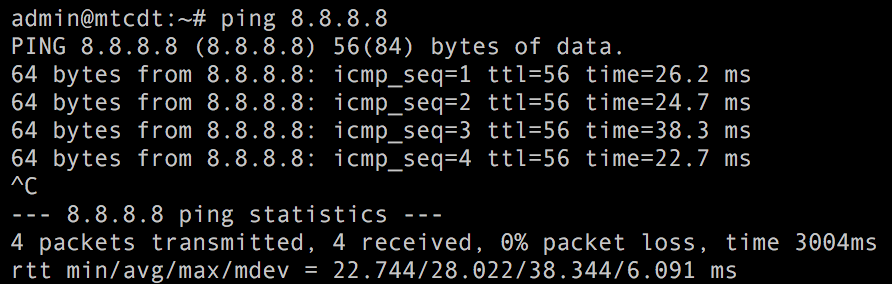
\includegraphics[width=0.5\textwidth]{figure/ping}
  \caption{The expected output of a \lstinline[language=sh]{ping 8.8.8.8} from the gateway.}
  \label{fig:ping}
\end{figure}

Additionally, as of the time of this writing, the \lstinline{config.h} file for the LMIC library is not configured for this use.
The necessary changes are as follows:
\begin{itemize}
\item Comment the line that says \lstinline[language=C]{#define CFG_eu868 1} and un-comment the line that says \lstinline[language=C]{#define CFG_us915 1}
\item Un-comment the line that says \lstinline[language=C]{#define DISABLE_INVERT_IQ_ON_RX}
\end{itemize}

%%% Local Variables:
%%% mode: latex
%%% TeX-master: "../writeup"
%%% End:
